\documentclass[aspectratio=169]{beamer}
% Modelo LaTeX para o PSE NE 2025.
% Desenvolvido por Silas Henrique (silash35@gmail.com),
% com contribuições de Daniel Diniz Santana (daniel.diniz@ufba.br).
% Versão 1.1.0 (21/11/2025)

% --- Outros Pacotes ---
\usepackage[T1]{fontenc}
\usepackage[utf8]{inputenc}
\usepackage[brazilian]{babel}

\usepackage{xkeyval}

% --- Pacotes gráficos e matemáticos ---
\usepackage{amsmath}       % Recursos avançados de matemática
\usepackage{esdiff}        % Facilita escrita de derivadas (\diff, \pdiff)
\usepackage[version=4]{mhchem} % Escrever fórmulas químicas e reações
\usepackage{tikz} % Desenhos

% --- Bibliografia ----
\usepackage[alf]{abntex2cite}
% Correção: força tamanho normal nas citações
%\renewcommand{\cite}[1]{\normalsize\oldcite{#1}}
%\let\oldcite\cite

% --- Configurações ---
\usebackgroundtemplate{
  
\includegraphics[page=2,width=\paperwidth,height=\paperheight]{background.pdf}
} % Plano de fundo
\usepackage[scaled=0.92]{helvet} % Fonte Helvetica

% --- Cores personalizadas ---
\definecolor{PSEblue}{HTML}{364971} % azul principal
\definecolor{PSEgray}{HTML}{757575} % cinza para rodapé e detalhes

% --- Configurações do Beamer ---
\usetheme{Copenhagen} % Tema geral
\setbeamertemplate{navigation symbols}{} % remove ícones de navegação
\setbeamertemplate{headline}{}           % esconde barra de topo
\setbeamertemplate{caption}[numbered]    % legendas numeradas

\usecolortheme[named=PSEblue]{structure}

\AtBeginSection[]{\frame{\sectionpage}}  % slide automático de seção

% Capa personalizada
\setbeamertemplate{title page}{
  \begin{center}
    \vspace{5mm}
    {\huge\textbf{\textcolor{PSEblue}{\inserttitle}}}

    \vspace{4mm}
    \insertauthor

    \vspace{2mm}
    \insertinstitute

    \vspace{4mm}
    \insertdate
  \end{center}
}

\setbeamertemplate{section page}{
  \begin{centering}
    \vfill
    \begin{beamercolorbox}[rounded=true,shadow=false,center,
        wd=\textwidth, % largura da caixa
        sep=10pt,      % espaçamento interno
        colsep*=1pt,   % espaçamento da borda
      ]{section title}
      \usebeamerfont{section title}\insertsection
    \end{beamercolorbox}
    \vfill
  \end{centering}
}

% Título dos slides
\setbeamercolor{frametitle}{fg=PSEblue}
\setbeamerfont{frametitle}{size=\LARGE, series=\bfseries}
\setbeamertemplate{frametitle}{
  \vspace{5mm}
  \hspace{-5mm}
  \insertframetitle
  \par
}

% Rodapé com numeração simples
\setbeamertemplate{footline}{%
  \begin{beamercolorbox}[wd=\paperwidth,ht=2.5ex,dp=1ex,rightskip=0.5cm]{footline}
    \hfill
    {\small \color{PSEgray}\insertframenumber{} / \inserttotalframenumber}
  \end{beamercolorbox}
  \vspace*{4mm}
}


% Configurações da apresentação
\title{Exemplo de Título de Trabalho, Escrito com as Palavras Iniciando com Letras Maiúsculas (Title Case)}

\author{Nome do Autor 1, Nome do Autor 2, Nome do Autor 3, ...}

\institute{Instituição dos autores}

\begin{document}

% Configurações do slide de capa
{
\setbeamertemplate{footline}{}
\usebackgroundtemplate{
  
\includegraphics[page=1,width=\paperwidth,height=\paperheight]{background.pdf}
}
\maketitle
}

% Inserindo o conteúdo principal da apresentação
% O comando \input{arquivo} permite separar o código em vários arquivos.
% Isso deixa o projeto mais organizado e facilita a manutenção,
% pois cada seção ou conjunto de slides pode ficar em um arquivo separado.
\section{Introdução}

\begin{frame}{\LaTeX\ Básico}
  No \LaTeX{} você pode escrever textos normalmente, e o compilador cuida da formatação.

  \vspace{2mm}

  Para enfatizar palavras, use:
  \begin{itemize}
    \item \texttt{\textbackslash textbf\{negrito\}} $\rightarrow$ \textbf{negrito}
    \item \texttt{\textbackslash textit\{itálico\}} $\rightarrow$ \textit{itálico}
    \item \texttt{\textbackslash underline\{sublinhado\}} $\rightarrow$ \underline{sublinhado}
  \end{itemize}

  \vspace{4mm}

  E use \texttt{\textbackslash begin\{itemize\}} para criar listas como esta.
\end{frame}

\begin{frame}{Equações no \LaTeX}

  O \LaTeX{} permite escrever equações matemáticas de forma clara.
  Por exemplo, uma equação diferencial pode ser escrita como:

  \begin{equation}
    \diff{h}{t} = \frac{1}{A}\left(q_{\text{in}} - q_{\text{out}}\right)
    \label{eq:tank}
  \end{equation}

  \vspace{4mm}

  Também existe suporte para componentes químicos usando o pacote \texttt{mhchem}, permitindo escrever diretamente no texto nomes como \ce{H2O}, \ce{CO2}, \ce{O2} e \ce{CH4}.

  \vspace{2mm}

\end{frame}

\begin{frame}{Citações no \LaTeX}

  Para incluir referências bibliográficas, basta adicionar sua entrada no arquivo \texttt{bibliografia.bib} e citar no texto.

  \vspace{4mm}

  Você pode citar assim:

  De acordo com \citeonline{araujo_2025}, a operação eficiente do gas lift depende de um controle preciso da injeção de gás.

  \vspace{2mm}

  Ou assim:

  A operação eficiente do \textit{gas-lift} depende de um controle preciso da injeção de gás \cite{araujo_2025}.

  \vspace{2mm}

  A seção de bibliografia é gerada automaticamente no final do slide.
\end{frame}

\section{Tabelas e Figuras}

\begin{frame}{Tabelas}
  Você pode usar tabelas, tal como a Tabela \ref{tab:parametros}.

  \vspace{2mm}

  \begin{table}[h]
    \centering
    \begin{tabular}{l c c}
      \hline
      Parâmetro   & Valor & Unidade                 \\
      \hline
      Pressão     & 5.0   & bar                     \\
      Temperatura & 298   & K                       \\
      Vazão       & 12.5  & \(\text{m}^3/\text{h}\) \\
      \hline
    \end{tabular}
    \caption{Parâmetros operacionais básicos}
    \label{tab:parametros}
  \end{table}
\end{frame}

\begin{frame}{Figuras}
  Você pode incluir figuras facilmente, como mostrado na Figura \ref{fig:pendulo}.

  \vspace{2mm}

  \begin{figure}[h]
    \centering
    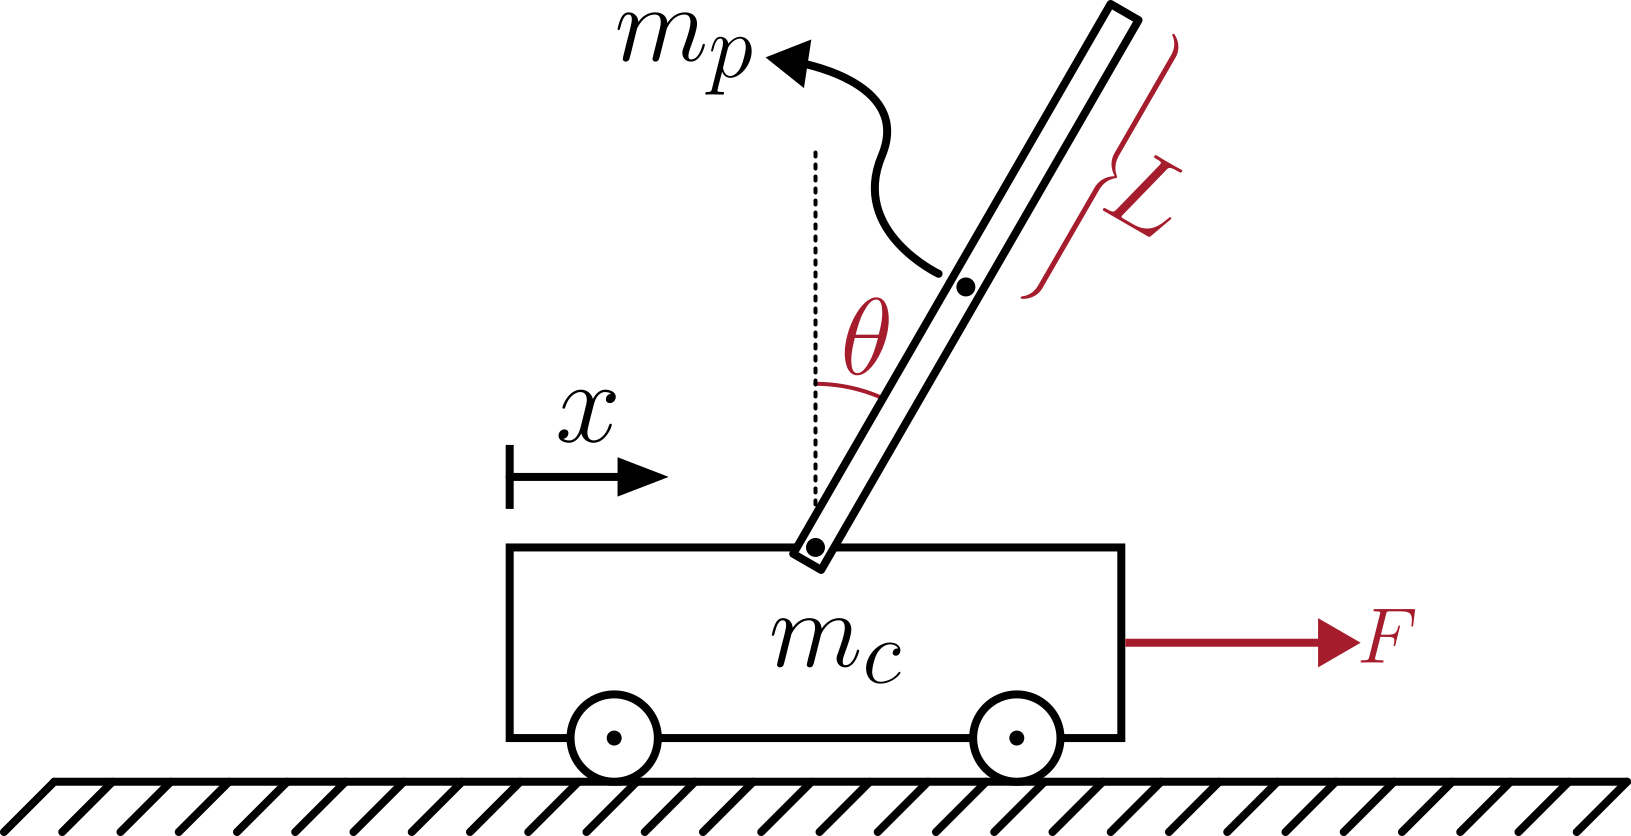
\includegraphics[width=0.6\textwidth]{figures/example.png}
    \caption{Representação do sistema físico de um pêndulo invertido.}
    \label{fig:pendulo}
  \end{figure}
\end{frame}


\begin{frame}{Agradecimentos}
  \centering \large Escreva aqui os agradecimentos do trabalho. Inclua instituições, agências de fomento, colaboradores ou qualquer apoio recebido.
\end{frame}

\begin{frame}{Bibliografia}
  \bibliography{bibliografia.bib}
\end{frame}

\end{document}
